\documentclass[sigconf, review=false]{acmart}

\usepackage[utf8]{inputenc}
\usepackage{booktabs} % For formal tables
\usepackage{graphicx}
\graphicspath{{yuanzhong-imgs/}}
\usepackage{float}
\PassOptionsToPackage{hyphens}{url}
\usepackage{hyperref}
\usepackage{multirow}
\usepackage{caption}
\usepackage{subcaption}
\usepackage{gensymb}
\usepackage{textcomp}
\usepackage{xspace}

\let\OldTexttrademark\texttrademark
\renewcommand{\texttrademark}{\OldTexttrademark\xspace}%

%% template settings
\settopmatter{printacmref=false} % Removes citation information below abstract
\renewcommand\footnotetextcopyrightpermission[1]{} % removes footnote with conference information in first column


%% title and name
\begin{document}
\title{Mobile \& Wireless Systems Final Report}
\subtitle{Crypto4CRFID}

\author{Yuanzhong Xia}
\affiliation{
  \institution{The University of Adelaide}
  \city{Adelaide}
  \state{SA}
  \postcode{5005}
}
\email{a1700831@student.adelaide.edu.au}

% ---------
%% abstract
% ---------
\begin{abstract}
    This report firstly introduces the background and motivation of this project, which is to build a secure CRFID system.
    Then, our system overview, system components and my contributions are mentioned in detail.
    My contribution include the lightweight block cipher algorithm study, hash function study and optimization study.
    Besides, others' related works on cryptanalysis, hash function cryptanalysis are mentioned as well.
    In the end, there are conclusions and my reflections about the whole project.
\end{abstract}
\keywords{Embedded System, RFID, Encryption, Hash, MSP430, Optimization, Security}
\maketitle


% --------------
%% main contents
% --------------

% Excellent introduction and motivation of the project, clearly outlining the potential of the work.
\section{Introduction and Motivation}
Radio Frequency Identification (RFID) technologies have been widely used in our daily lives:
student cards, contactless payment, object tracking (like airport baggages, express packages and experimental animals),
item identification, distributed wireless sensor networks used for environment monitoring, etc. \cite{wikipedia2017rfid}
They are normally built with Application Specific Integrated Circuits (ASIC).

Unlike RFID, Computational RFID (CRFID) that our studies are based on has an ultra low power microcontroller (MCU),
thus it has a firmware software which we can specifically modify for our applications.
The firmware follows the EPC\texttrademark Radio-Frequency Identity Protocols Class-1 Generation-2 UHF RFID version 2\cite{epcglobal2013}.
This standard defines how a tag is captured by a reader, and how information are transmitted between reader and tag.
It also contains several custom security extension commands for developers to use in their implementations.

However, CRFID has a limited amount of computational resources, which determines that it is unlikely to apply
modern high-computational-complex encryption algorithms (like RSA algorithm) on it.
Therefore, to build a security system becomes a crucial problem in research area.

In this project, we mainly try to build a secure CRFID system
% Not implemented: the CRFID tag can verify a reader's legitimacy and
where the reader can identify a CRFID's legitimacy.
After passing the two-way verification, they can transfer the critical data securely.

\subsection{Devices}
In this project, we use WISP 5 \footnote{WISP5 - WISP Home: \url{https://wisp5.wikispaces.com/WISP+Home}.} (shown in Figure \ref{fig-wisp5})
as the CRFID experimental device.
It contains a Texas Instruments (TI) MSP430FR5969 MCU \footnote{MSP430\texttrademark FR5969 16 MHz Ultra-Low-Power MCU: \url{http://www.ti.com/product/MSP430FR5969}.}
which uses 16-bit architecture with up to 16‑MHz Clock, and has 2 KB Static Random Access Memory (SRAM) and 64 KB Ferroelectric RAM (FRAM).

\begin{figure*}
\centering
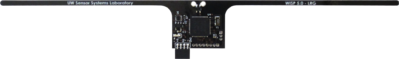
\includegraphics[width=0.6\textwidth]{wisp5.png}
\caption{WISP 5 CRFID.}
\label{fig-wisp5}
\end{figure*}

The firmware is run by the MSP430 MCU. Hence, I only need to test algorithms on MSP430RF5969 no matter what CRFID I use.
Moreover, we have only one WISP 5, and another team member needs it to test the communication between CRFID and reader.
Therefore, I use another MSP430FR5969 come with MSP430FR5969 LaunchPad Development Kit
\footnote{MSP-EXP430FR5969 MSP430FR5969 LaunchPad Development Kit: \url{http://www.ti.com/tool/MSP-EXP430FR5969}.}
shown in Figure \ref{fig-launchpad}.

\begin{figure}
\centering
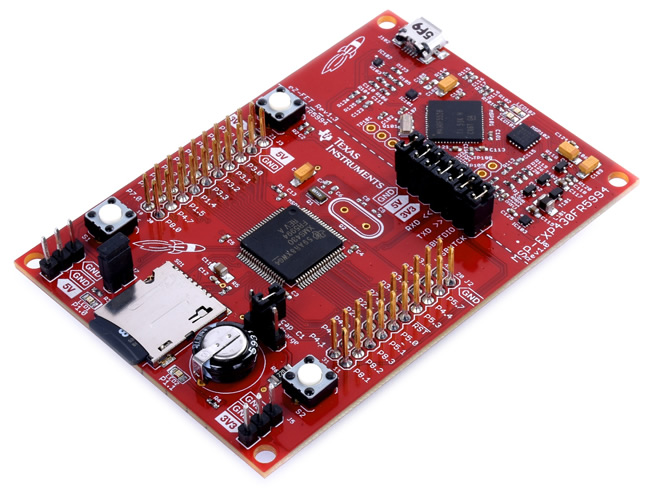
\includegraphics[width=0.4\textwidth]{launchpad.jpg}
\caption{MSP430FR5969 LaunchPad.}
\label{fig-launchpad}
\end{figure}

For debugging, there is no difference theoretically, plus, it provides some additional useful tools
like EnergyTrace++\texttrademark which can trace MCU current consumption.
As a result, all my experiments in this project are tested on this LaunchPad.

\subsection{System Overview}
The whole system architecture is shown in Figure \ref{fig-arch}.
This system contains two components: PC client and WISP 5.

\begin{figure*}
\centering
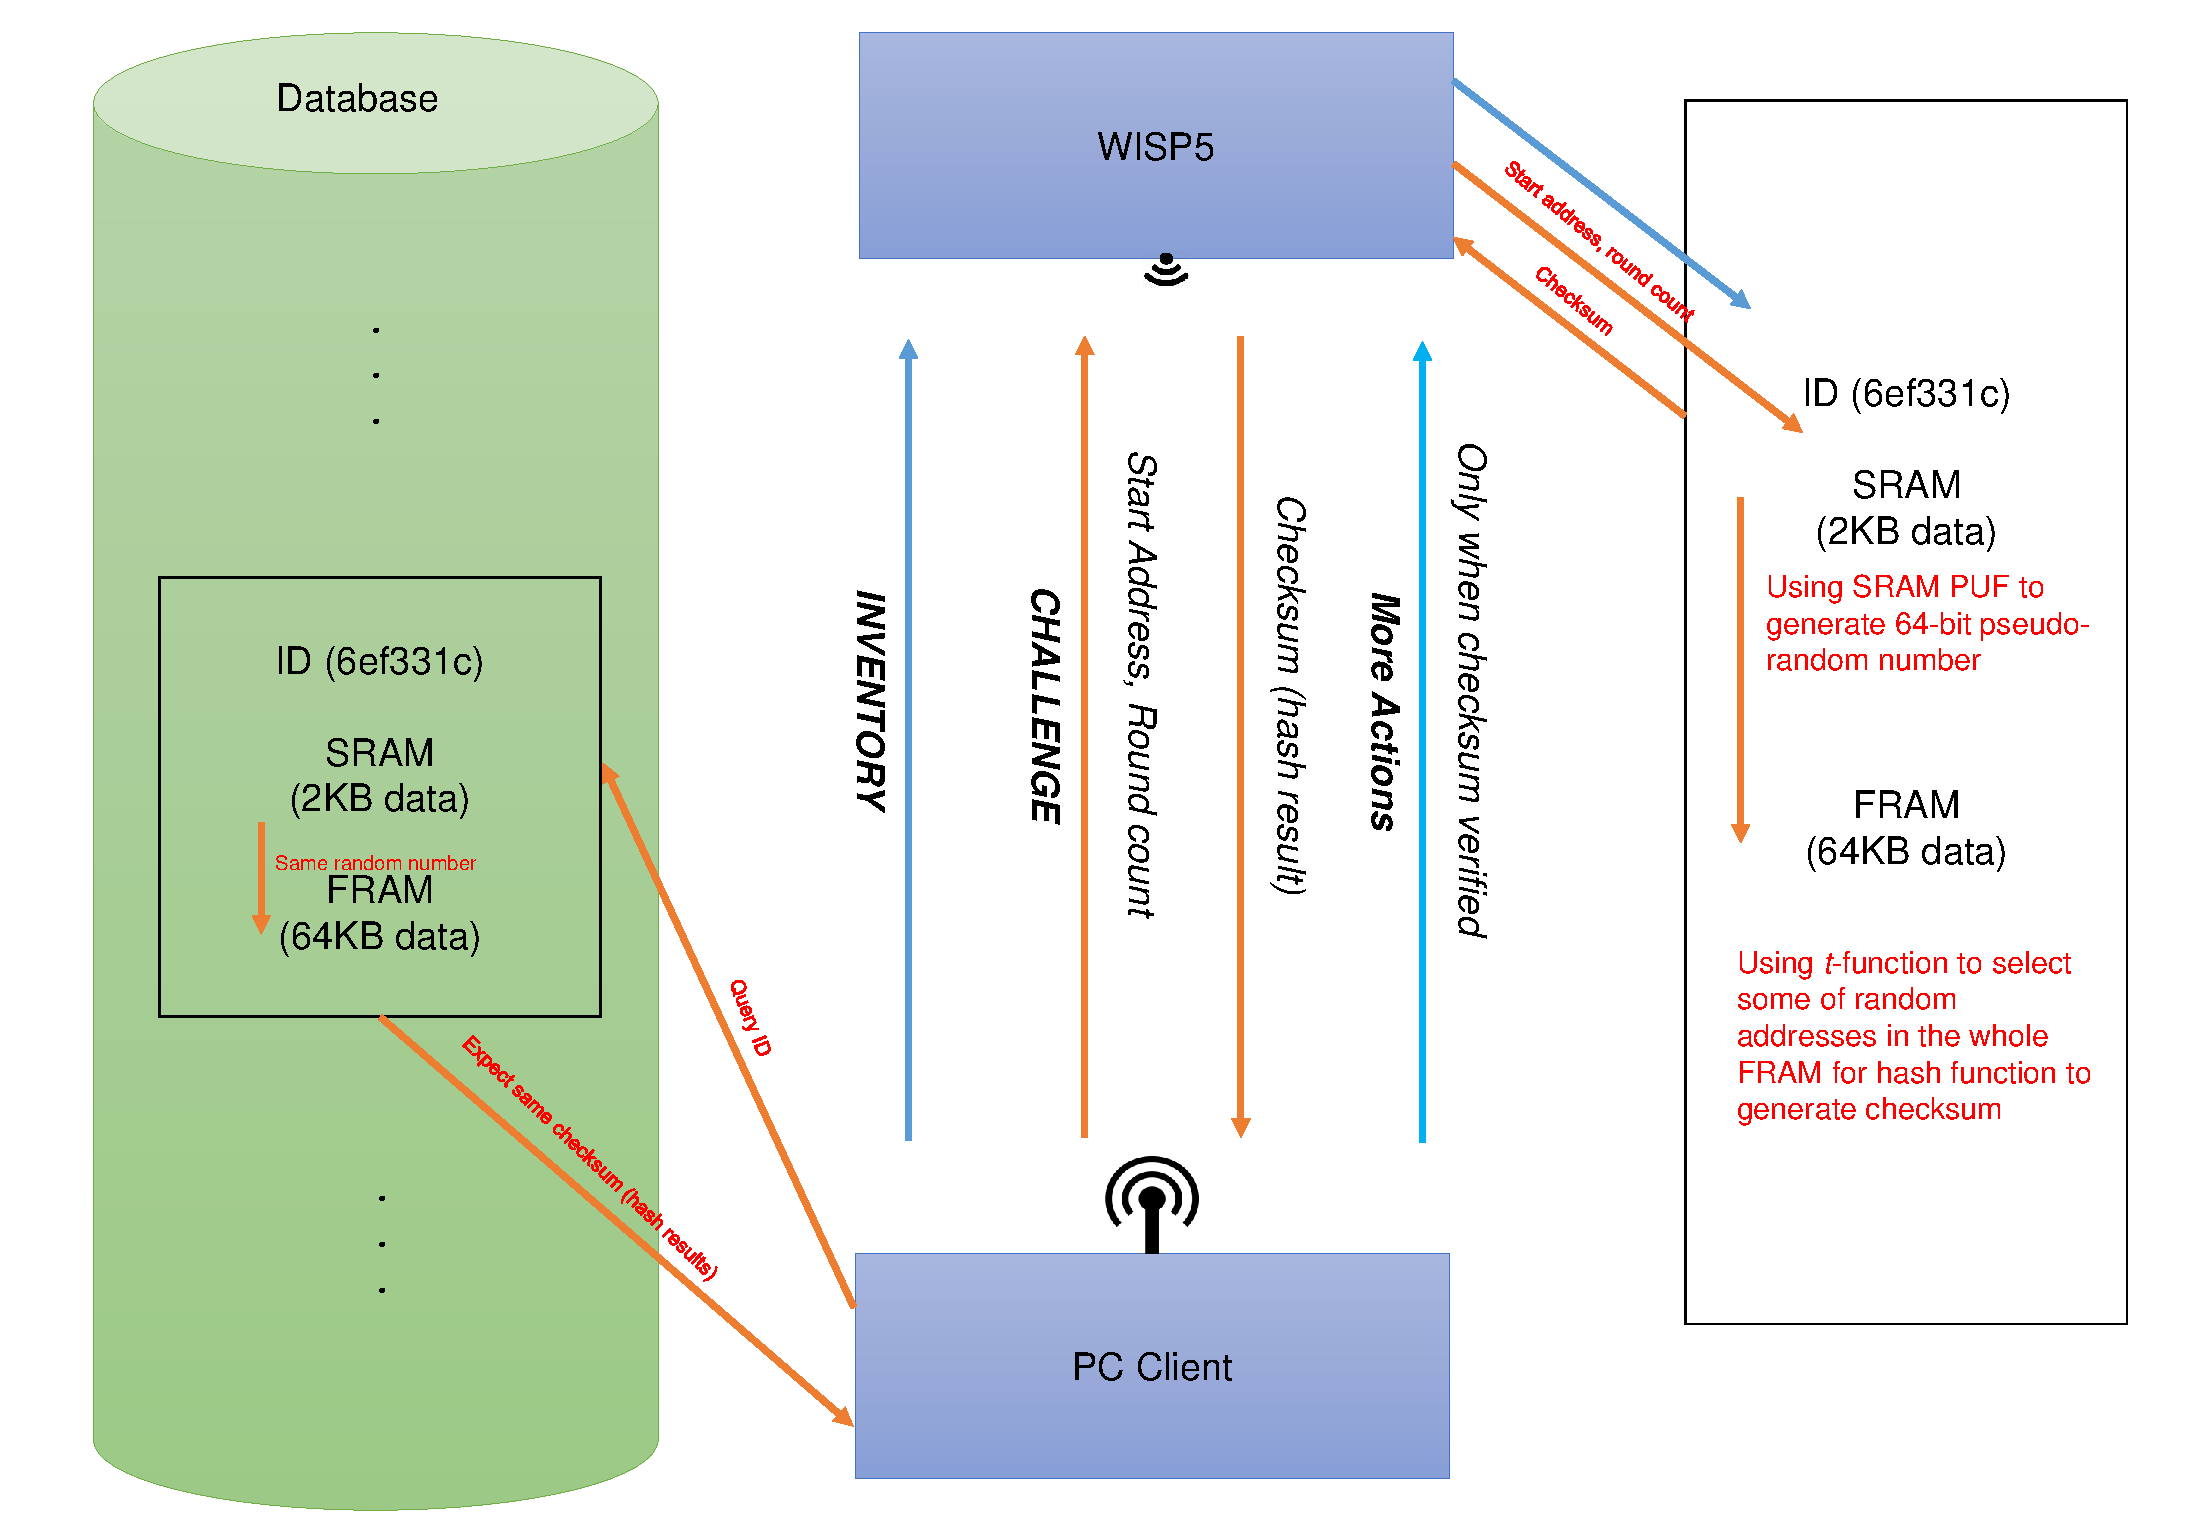
\includegraphics[width=0.7\textwidth]{arch.pdf}
\caption{System architecture.}
\label{fig-arch}
\end{figure*}

PC client contains a database storing a copy of FRAM and SRAM signature
(used by Physical Unclonable Functions implemented by teammate Yang Su).
Each copy of FRAM and SRAM are indexed by unique EPC value.

WISP 5 is supposed to contain legit EPC value which is stored in PC's database,
legit firmware which will be verified by my hash function,
and legit SRAM signature which is used for generating real random number.

The communication between PC client and WISP 5 follows the EPCglobal standard,
the extended security command is implemented by teammate Sangyeol Kim.
When connection established, PC will send WISP 5 a challenge which contains the beginning address and the round count.
Round count is used together with \textit{t}-function (implemented by teammate Jingwen Shan),
which will be introduced in Section \ref{sec-int} in detail.
Once WISP 5 receives the challenge, it runs the hash function implemented by me to get a checksum and send it back to PC client;
Meanwhile, PC client uses the same hash function to calculate the checksum, and compare it with the received checksum.
If they matches, the WISP 5 is regarded as a legit one.

\section{Related Works}
\subsection{Lightweight Block Cipher Algorithms}
Papers on lightweight block cipher algorithms are mentioned in Section \ref{sec-block} in detail.
Hence, they are not discussed with related works.

Besides, there some benchmark survey papers on lightweight block cipher algorithms:

\begin{itemize}
    \item In 2013, Cazorla \textit{et al.} published a survey paper comparing the performance between
          many lightweight block cipher algorithms using an MSP430 simulator called ``mspdebug''.
          \footnote{mspdebug GitHub repository: \url{https://github.com/dlbeer/mspdebug}.} \cite{cazorla2013survey}
    \item In 2014, Buhrow \textit{et al.} published a survey paper comparing different implementations
          of selected lightweight block cipher algorithms. \cite{buhrow2014block}
    \item In 2015, Cazorla \textit{et al.} again published a new survey paper comparing the performance between
          a set of lightweight block cipher algorithms using a real MSP430FG4618 device. \cite{cazorla2015survey}
    \item In 2017, Hatzivasilis \textit{et al.} published a survey on more than 30 lightweight block cipher algorithms.
          They only did some benchmark because a part of the algorithms did not have reference implementations. \cite{hatzivasilis2017review}
\end{itemize}

However, the first three survey papers did not mention cryptanalysis of the selected block cipher algorithms.
The last paper mentioned the cryptanalysis, but it used the standard 8051 MCU and the ATtiny45, instead of MSP430.

Moreover, the two papers from Cazorla \textit{et al.} conflicts with each other.
As well, our experiment results on MSP430FR5969 are in conflict with Cazorla \textit{et al.}'s two papers.
That is also one of the project's motivations.

\subsection{Hash Functions}
As far as I know, there is no cryptographic hash function survey researches from 2010.
A most-cited one is survey paper from Bakhtiari \textit{et al.} in 1995 \cite{bakhtiari1995cryptographic}.
The functions they discussed in that paper are MD2, MD4, MD5 and SHA-1.
However it is not useful now because all those discussed functions are full attacked:

\begin{itemize}
    \item MD2 was shown to be vulnerable for collision by Muller in 2004,
          using a preimage attack with a time complexity equivalent to $2^{104}$. \cite{muller2004md2}
    \item MD4 was fully collided using cheap computational cost by Leurent
          using preimage attack in a time complexity of $2^{102}$ in 2008. \cite{leurent2008md4}
    \item MD5 has been proved its distribution is not safe since 2004 \cite{hawkes2004musings}.
          Later in 2013, Xie \textit{et al.} published a method for a very quick collision attack \cite{xie2013fast},
          which takes less than a second to attack it on a regular computer.
    \item SHA-1 was also fully proved to be vulnerable for collision, using multi-block collision techniques
          by Wang \textit{et al.} since 2005. \cite{wang2005finding}
\end{itemize}

Besides, there are many cryptographic hash function papers using block ciphers to construct hash functions.
However, nearly all of the block ciphers are with key and block of same sizes.
I can hardly find a paper constructing a hash function constructed using key and block of different sizes.
This is not really helpful because the block ciphers we study are with various sizes of key and block.
Therefore, this is the reason why I refer to open-source projects to seek \textit{g}-functions used for constructions
in Section \ref{sec-one}.

\subsection{MSP430 Algorithm Optimization}
I have searched for ``assembly language'', ``MSP 430'' and ``Optimization'' key words on Google\texttrademark Scholar.
The only results that I can find are about factory assembly lines or sequences.

Additionally, the algorithms are evolutionary computation technologies. For example:

\begin{itemize}
    \item Dini \textit{et al.} derived a Genetic Algorithm to optimize assembling a simulated CAD product
          to find a better sequence that assembles quickly. \cite{dini1999generation}
    \item Haq \textit{et al.} derived a method to optimize load balance on assembly line
          using a hybrid genetic algorithm. \cite{haq2006hybrid}
\end{itemize}

Above all, as far as I know, there is on manual code optimization researches
on assembly programming language or MSP430 programming.
Therefore, I referred to some online materials which are mentioned in Section \ref{sec-low}.


\section{Lightweight Block Cipher Algorithm} \label{sec-block}


\section{Hash Functions}
\subsection{One-way Compression Functions} \label{sec-one}
// TODO: constructions

// TODO: g-functions

\subsection{Cryptographic Hash Function}

\subsection{Pure Hash Function}

\subsection{Benchmark}

\subsection{Integration with Whole System} \label{sec-int}



\section{Optimization}

\subsection{Compiler Optimization}

\subsection{High-Level Programming Language Optimization}

\subsection{Low-Level Programming Language Optimization} \label{sec-low}
// TOOD: online materials




// TODO: feedback from writing centre

\section{Conclusion}


% -----------

\bibliographystyle{ACM-Reference-Format}
\bibliography{ref}

\end{document}
